\documentclass[11pt,a4paper]{article}
\usepackage{fontspec}
\setmainfont{TeX Gyre Pagella}
\newfontfamily\headfont{Inter}[UprightFont=*-ExtraBold,BoldFont=*-ExtraBold,Extension=.otf,Path=/usr/share/fonts/opentype/inter/]
\usepackage[a4paper,margin=2.3cm]{geometry}
\usepackage{graphicx,booktabs,float,caption,array,xcolor,longtable}
\usepackage{xurl}
\usepackage[hidelinks]{hyperref}
\usepackage{titlesec}
\usepackage[round]{natbib}
\usepackage{setspace}
\setstretch{1.05}
\renewcommand{\topfraction}{0.9}
\renewcommand{\bottomfraction}{0.8}
\renewcommand{\textfraction}{0.1}
\renewcommand{\floatpagefraction}{0.75}
\setlength{\parindent}{0pt}
\setlength{\parskip}{0.55em}
\titleformat{\section}{\headfont\Large}{\thesection}{0.8em}{}
\titleformat{\subsection}{\headfont\large}{\thesubsection}{0.8em}{}
\captionsetup{font=small,labelfont=bf}
\urlstyle{same}
\hypersetup{pdftitle={Named After Somewhere Else},pdfauthor={Tristan Hotham}}

\begin{document}
\begin{center}
{\Large\bfseries Named After Somewhere Else\par}
\vspace{0.4em}
{\large Places named after other places in Wikidata: what they borrow,\\how far the names travel, and who gave names to whom\par}
\vspace{1.2em}
{\large Tristan Hotham\par}
\vspace{0.3em}
{\small Independent researcher\\
ORCID: 0000-0003-4931-9349\\
DOI: https://doi.org/10.5281/zenodo.23878606\par}
\vspace{0.8em}
2026
\end{center}

\begin{quote}
\small
\begin{center}\textbf{Abstract}\end{center}
I map every human settlement that Wikidata records as ``named after'' (P138) another geographical place, joining each to its namesake with a great circle. After removing census and statistical areas, camps, stations and other entries that are not settlements in the ordinary sense, 3,981 links remain, from 3,837 places to 3,551 namesakes. Only 37\% of the links are to other settlements; the rest are to rivers (14\%), mountains and hills, lakes, coasts, buildings, regions and countries. The distances are bimodal: the median is 4.4 km and 58\% are under 10 km, yet 22\% exceed 1,000 km and 14.2\% join different landmasses. 22\% cross a national border; the United Kingdom is the source of 29\% of these, 96\% of them to the United States, Australia, Canada and New Zealand. The most borrowed namesakes are Prague (13 places, mostly Czech suburbs) and Amsterdam (10, mostly abroad). 75 places are a ``New X'' named after X, more than half within 30 km of it. Coverage is very uneven: four countries hold 54\% of all links and Latin America only 2.2\%, so the file records where Wikidata's editors have entered name origins as much as where names travelled.

\textbf{Keywords:} toponymy; place names; Wikidata; migration; colonial settlement; geography of naming; open data; mapping
\end{quote}

\section{Introduction}
Toponymy, the study of place names, has long recognised that many names are transferred: settlers, soldiers and planners give a new place the name of an old one, so that one name ends up on two continents. Transfer names are a familiar feature of the colonial and settler world, from the English names of New England and Australia to the Dutch names of New Netherland, and they are one of the few traces of migration written on the map itself. They are usually studied country by country, from gazetteers and local histories. Wikidata, the collaborative knowledge base behind Wikipedia, now records name origins for many places in a structured way through its ``named after'' property (P138), which makes a first global look possible. This paper takes every settlement that Wikidata says is named after another geographical place and asks simple questions: what kinds of places lend their names, how far the names travel, which countries give and receive names, and how far the answers are shaped by Wikidata's own coverage. An interactive map accompanies the paper at \url{https://maps.tristanhotham.com/named-after/}.

\section{Data and methods}
\subsection{The query}
The data come from a single SPARQL query against Wikidata, run on the QLever engine \citep{qlever} in 2026. It returns every item that is an instance of human settlement (Q486972) or any of its subclasses and has a ``named after'' value that is an instance of geographic location (Q2221906) or any of its subclasses, where both have coordinates (P625) and English labels; with the countries (P17) of both, the population (P1082) and inception (P571) of the settlement where known, and each class (P31) of the namesake. Because every combination of multiple values produces a row, the 23,818 rows collapse to 7,666 distinct links between 7,136 places and 6,812 namesakes. A place keeps its first coordinates in the result, its largest population and its earliest inception; a namesake keeps its first coordinates and all its classes. Wikidata content is in the public domain (CC0).

\subsection{What counts as a settlement}
Wikidata's settlement class is broad, and the raw result contains many items that are not settlements in the ordinary sense. I removed them by their English labels (Table~\ref{tab:excl}). By far the largest group is the US Census Bureau's urban areas and other statistical areas, which Wikidata records as named after their principal town and which would therefore count every such town twice. I also removed megalopolises and conurbations, regions and counties, concentration, extermination, prison and internment camps, stations, bases and ranger posts, parks and ski resorts, links from an item to itself, and ``administrative twins'': a place with the same name as a settlement or region namesake less than 30 km away, typically a municipality and the town it is named after. In all 3,684 links (48\%) were removed. Cities, towns, villages, hamlets, townships, suburbs, neighbourhoods, housing estates and city districts are kept.

\begin{table}[tbp]\centering\small\caption{Links removed from the raw query result, in the order the rules are applied.}\label{tab:excl}\begin{tabular}{p{10.5cm}rr}\toprule Rule & Places & Links\\\midrule
Links from a place to itself & 13 & 13\\
Census and statistical areas (urban, metropolitan, micropolitan, combined statistical areas) & 2,924 & 3,295\\
Megalopolises, conurbations, agglomerations and 'Greater' areas & 18 & 24\\
Regions, counties, provinces and new areas & 7 & 10\\
Camps that were not homes (concentration, extermination, prison, internment, DP and military camps) & 15 & 15\\
Stations, airports, bases and ranger posts & 64 & 66\\
Parks, resorts, ski areas and industrial estates & 15 & 18\\
Administrative twins (same name, under 30 km) & 243 & 243\\
\midrule All removed & & 3,684\\ Kept & 3,837 & 3,981\\\bottomrule\end{tabular}\end{table}

\subsection{What the namesake is}
The query returns the namesake's classes as bare identifiers, 1,199 of them. I read each common class from the namesakes that carry it (for example, the namesakes of class Q4022 are Buffalo River, the Lahn and the River Dee, so it is ``river'') and listed it under one of four categories: settlement, river, region or country, and mountain or hill. A namesake with any settlement class counts as a settlement (Manhattan, an island and a borough, is a settlement); otherwise region, then river, then mountain. 78\% of namesakes were sorted by a listed class. The remainder were sorted by a word in the name (River, Mount, County), counted as a settlement if they appear in the file as settlements themselves, or otherwise placed in ``other'', a residual that holds lakes, coasts and islands, buildings, streets, parks and features of every kind.

\subsection{Distances, countries and landmasses}
Distances are great-circle distances between the two Wikidata coordinate pairs. For a river, a region or a mountain range Wikidata gives one point, sometimes the mouth, the source or a centre, so distances to such namesakes are indicative only. Countries are Wikidata's own (P17), matched to Natural Earth \citep{naturalearth} by Natural Earth's Wikidata identifiers; where Wikidata gives a historical state or no country, I used the Natural Earth country containing the point. Wikidata's country and the country containing the point agree for 98.8\% of places. A link crosses an ocean when its two ends lie on different landmasses: the Americas; Africa, Europe and Asia; Australia and its neighbours; Antarctica; and remote ocean islands. Each Natural Earth land polygon that is not one of the four continental masses is joined to the nearest of them if it lies within 2,500 km (so Britain, Japan, Newfoundland and New Zealand join their neighbours) and otherwise counts as a remote island.

\section{Results}
\subsection{What places are named after}
Table~\ref{tab:cats} and Figure~\ref{fig:types} show the namesakes by category. Only 1,484 links (37.3\%) are to another settlement. Rivers account for 570 (14.3\%), mountains and hills for 298, regions and countries for 235, and the residual for 1,394, of which 254 are lakes, reservoirs and seas. Counting rivers, mountains, lakes, coasts, forests and valleys together, 38.1\% of names come from the natural landscape. The kind of namesake largely determines the distance: the median is 2.4 km for mountains and hills, 12.8 km for rivers, 121.5 km for settlements and 1092.4 km for regions and countries.

\begin{table}[tbp]\centering\small\setlength{\tabcolsep}{4pt}\caption{Links by the kind of namesake: count, share, distinct namesakes, median distance (km), and the shares within 10 km, crossing a border and crossing an ocean.}\label{tab:cats}\begin{tabular}{lrrrrrrr}\toprule Namesake & Links & Share & Namesakes & Median km & $<$10 km & Border & Ocean\\\midrule
Settlement & 1,484 & 37.3\% & 1,246 & 121.5 & 43\% & 38\% & 28\%\\
River & 570 & 14.3\% & 524 & 12.8 & 45\% & 6\% & 1\%\\
Region or country & 235 & 5.9\% & 175 & 1,092.4 & 5\% & 58\% & 33\%\\
Mountain or hill & 298 & 7.5\% & 276 & 2.4 & 75\% & 9\% & 4\%\\
Other & 1,394 & 35.0\% & 1,330 & 0.9 & 83\% & 8\% & 4\%\\
\midrule All & 3,981 & 100\% & 3,551 & 4.4 & 58\% & 22\% & 14\%\\\bottomrule\end{tabular}\end{table}

\begin{figure}[tbp]\centering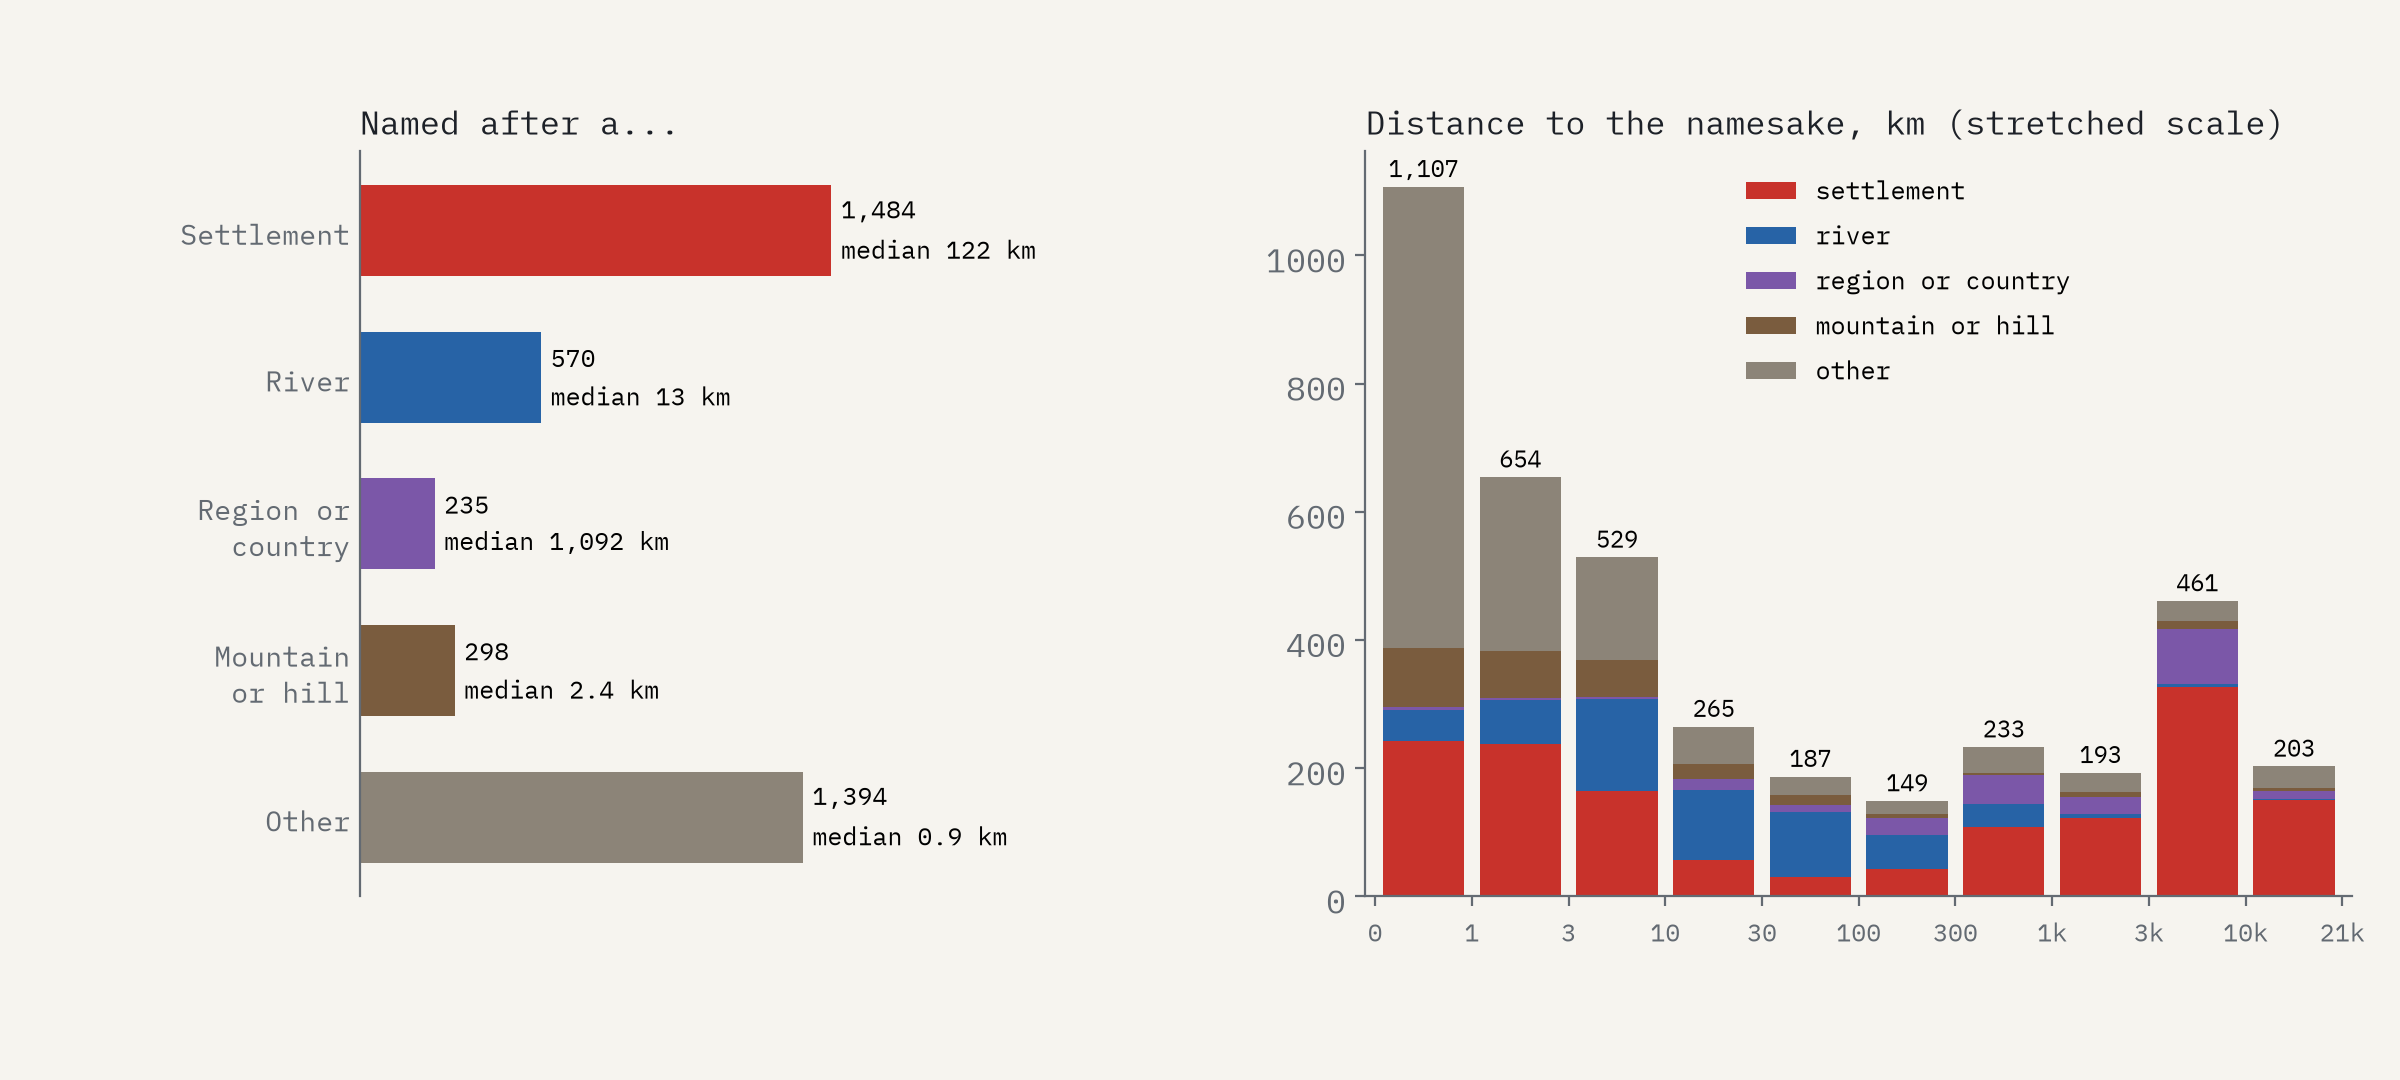
\includegraphics[width=\textwidth]{f_types.png}
\caption{Left: links by the kind of namesake, with the median distance. Right: links by distance from namesake to place, on a stretched scale, by kind of namesake.}\label{fig:types}\end{figure}

\subsection{How far names travel}
The median link is 4.4 km long; a quarter are under 0.8 km and three quarters under 504.1 km. 57.5\% are within 10 km. The distribution is bimodal (Figure~\ref{fig:types}, right): a large mode of neighbours, within a few kilometres, a trough between about 100 and 3,000 km, and a second mode of long-distance transfers, 587 links over 5,000 km and 203 over 10,000 km. 567 links (14.2\%) join different landmasses (Figure~\ref{fig:ocean}); 73.7\% of these are to settlements, and their median length is 7,620 km. Among all links to settlements, 28.2\% crossed an ocean. The longest links are British names in New Zealand: 14 of the fifteen longest end there, the longest 19,071 km from Lansdown to Lansdowne.

\begin{figure}[tbp]\centering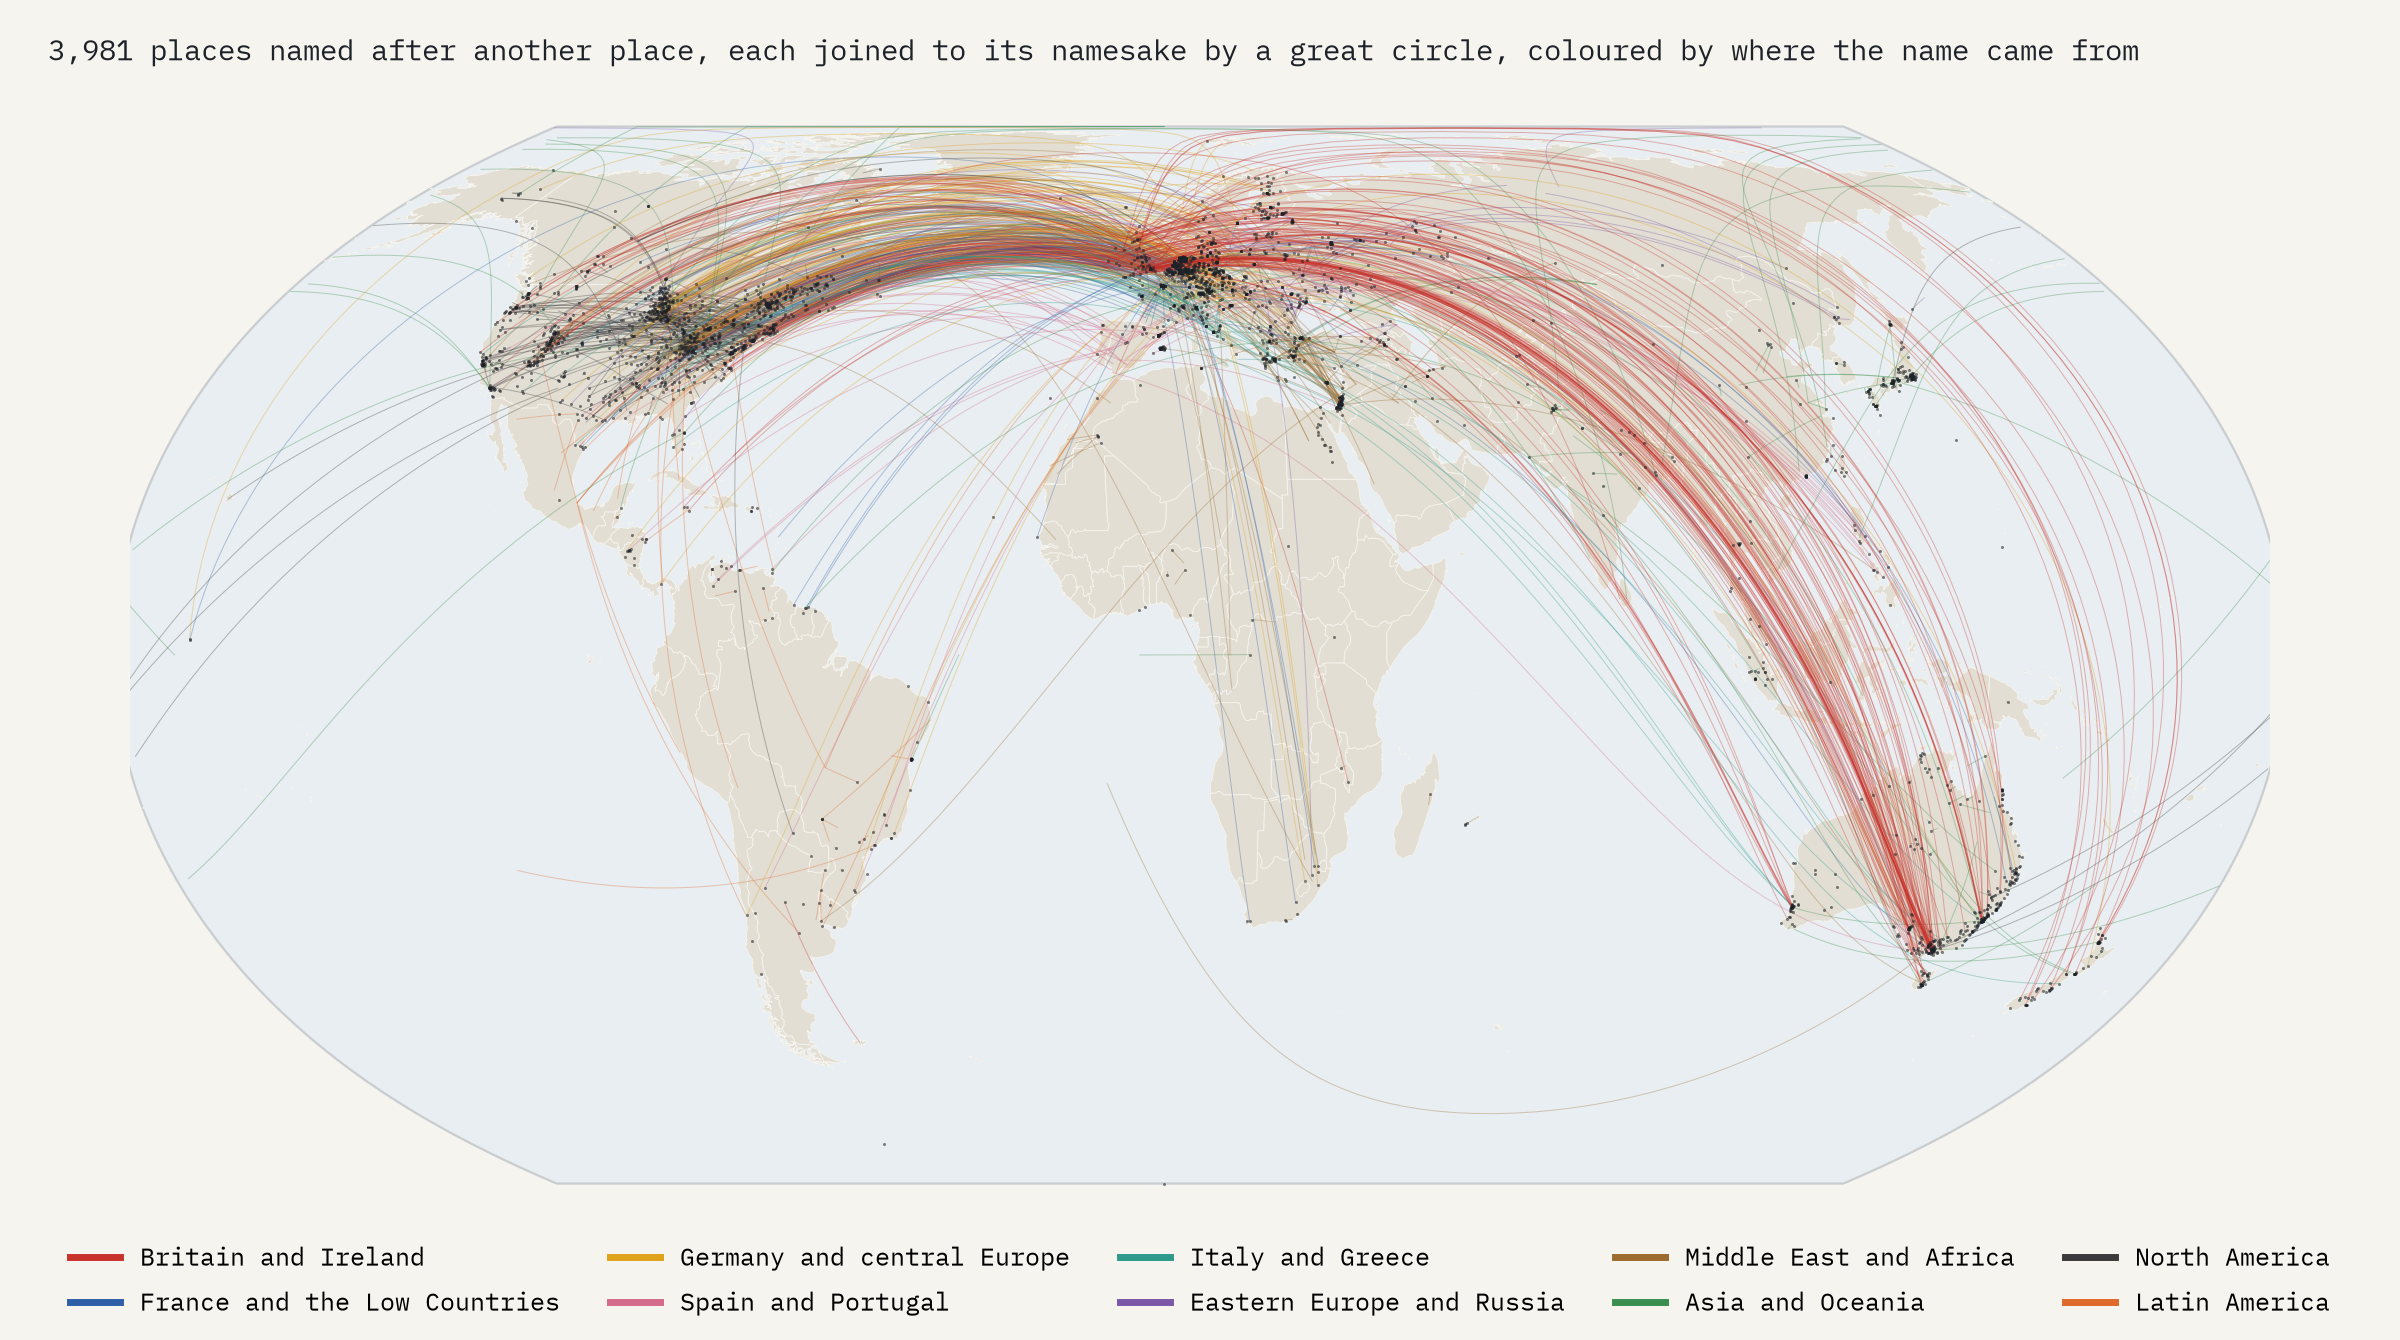
\includegraphics[width=\textwidth]{f_map.png}
\caption{Every link, as a great circle from the namesake to the place, coloured by the region of the namesake. Equal Earth projection, centred on 10\,E.}\label{fig:map}\end{figure}

\begin{figure}[tbp]\centering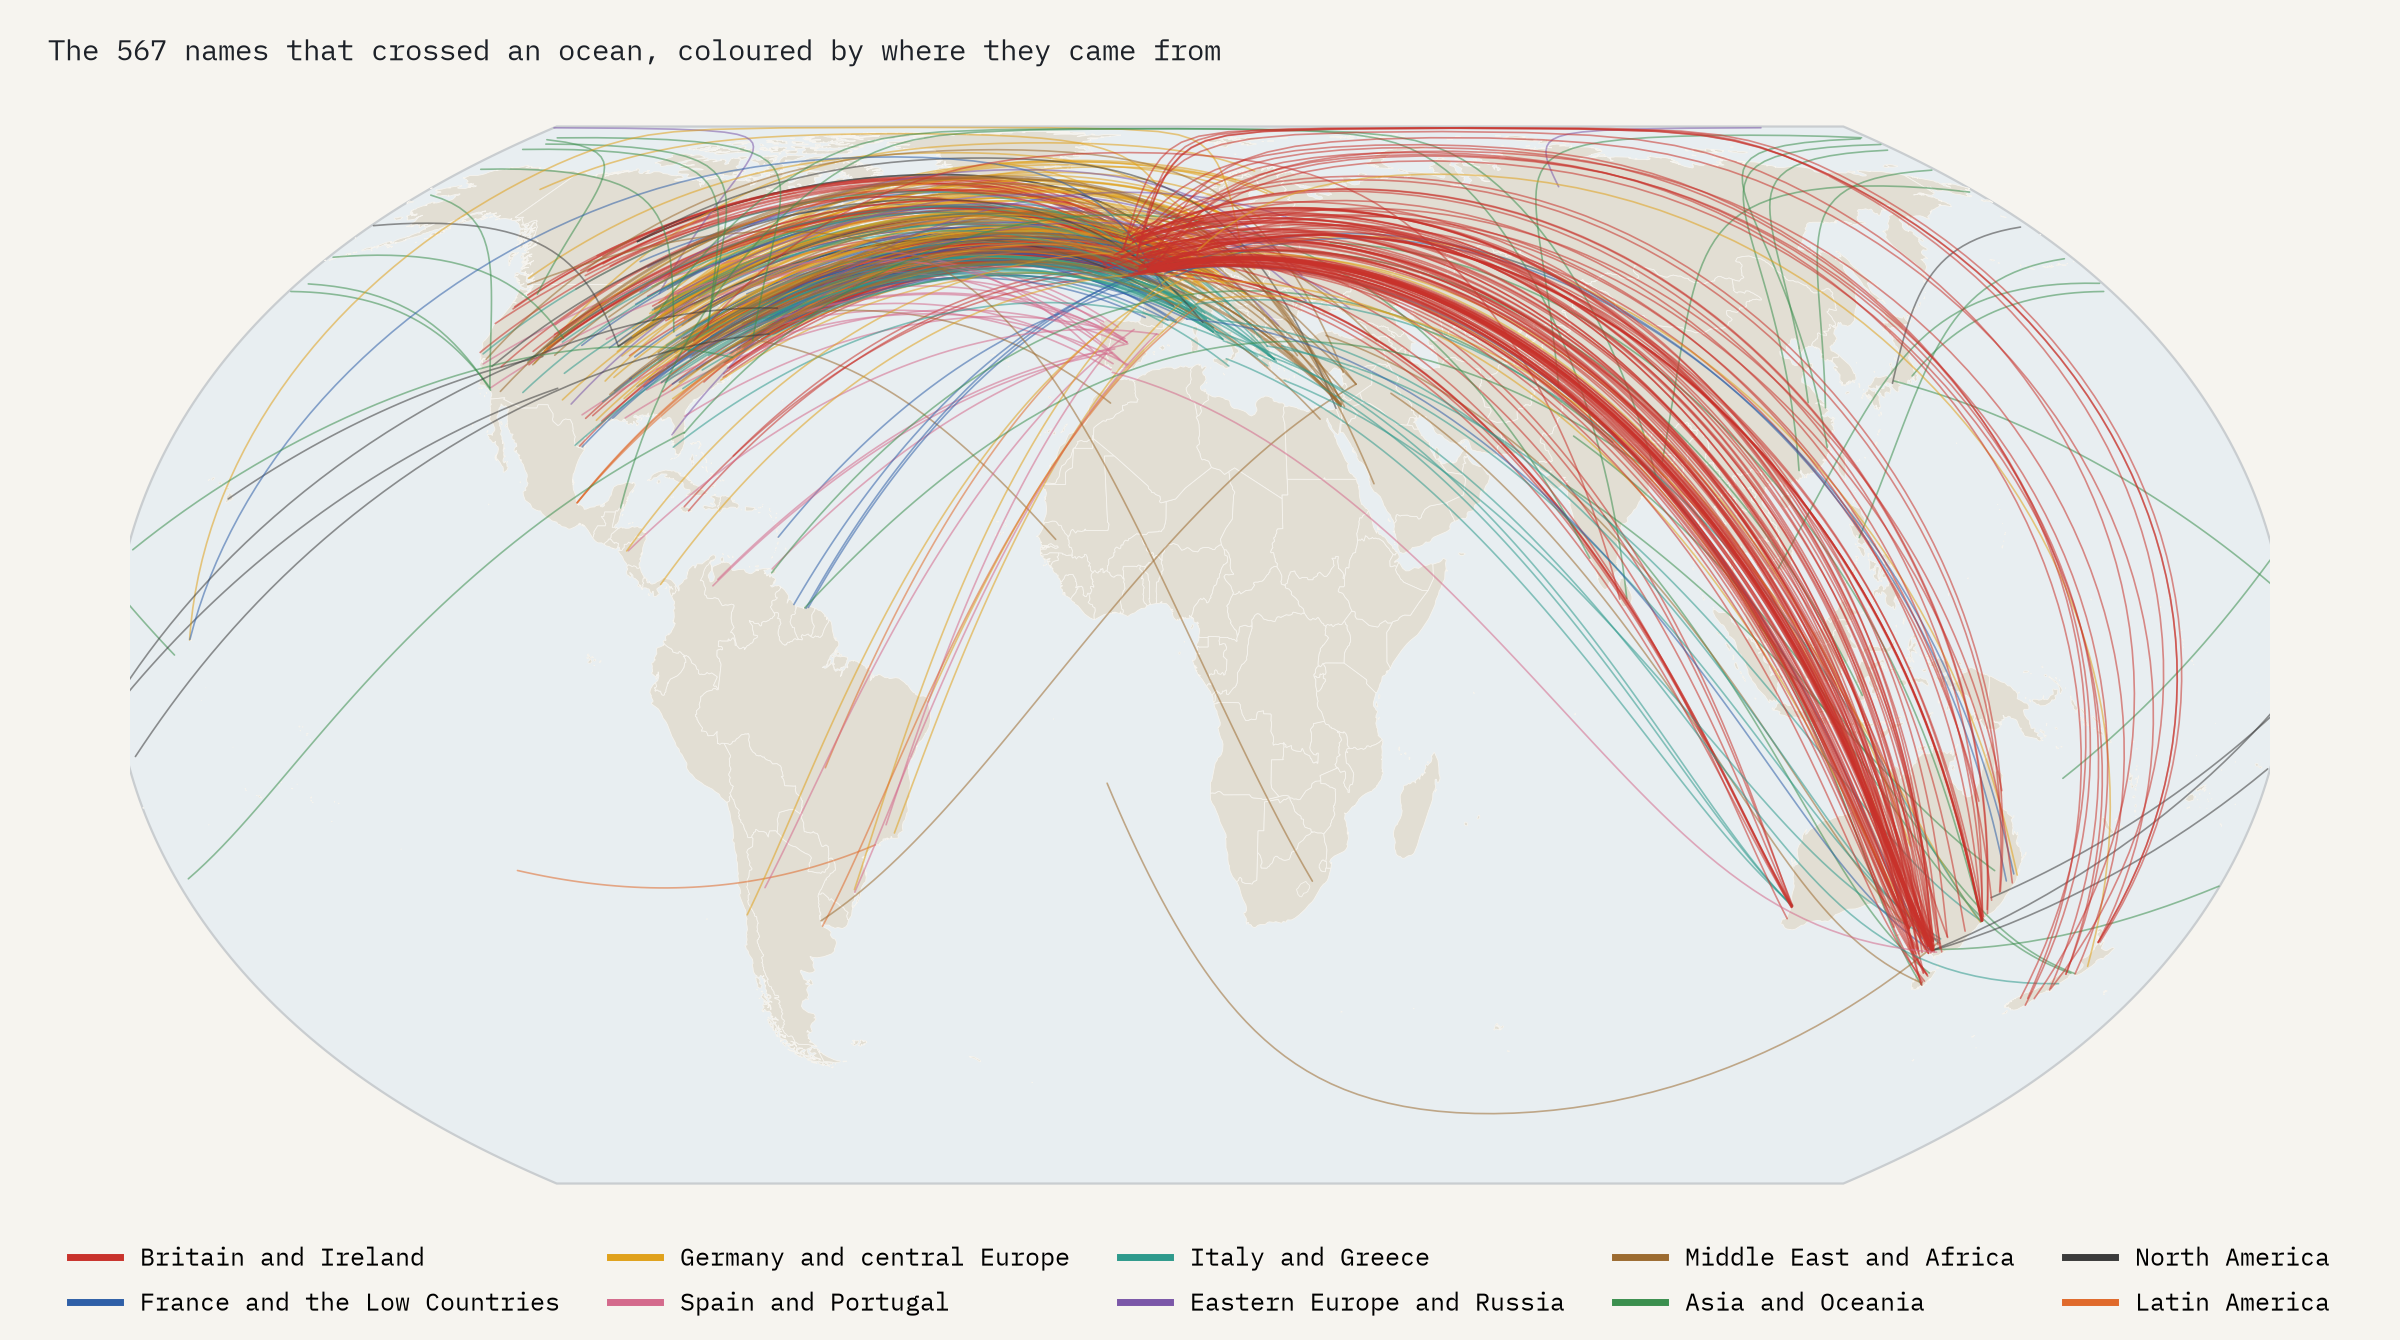
\includegraphics[width=\textwidth]{f_ocean_map.png}
\caption{The 567 links that join two different landmasses.}\label{fig:ocean}\end{figure}

\subsection{The most borrowed names}
Most namesakes lend their name once: 92.4\% have a single place named after them. The most borrowed is Prague, with 13 places, 10 of them in Czechia, most of them suburbs called Pražské Předměstí. Amsterdam has 10, 8 of them abroad, in the United States, Canada, Suriname, Guyana and South Africa (Figure~\ref{fig:top}). Moscow's 8 are mostly city districts. Berlin, Paris, Bristol, Windsor, Athens and Bethlehem each have four to six places, almost all abroad. Some of the most borrowed are not places in the narrow sense: ``Europe'' has 8, European quarters of several cities, and Anatolia 8.

\begin{figure}[tbp]\centering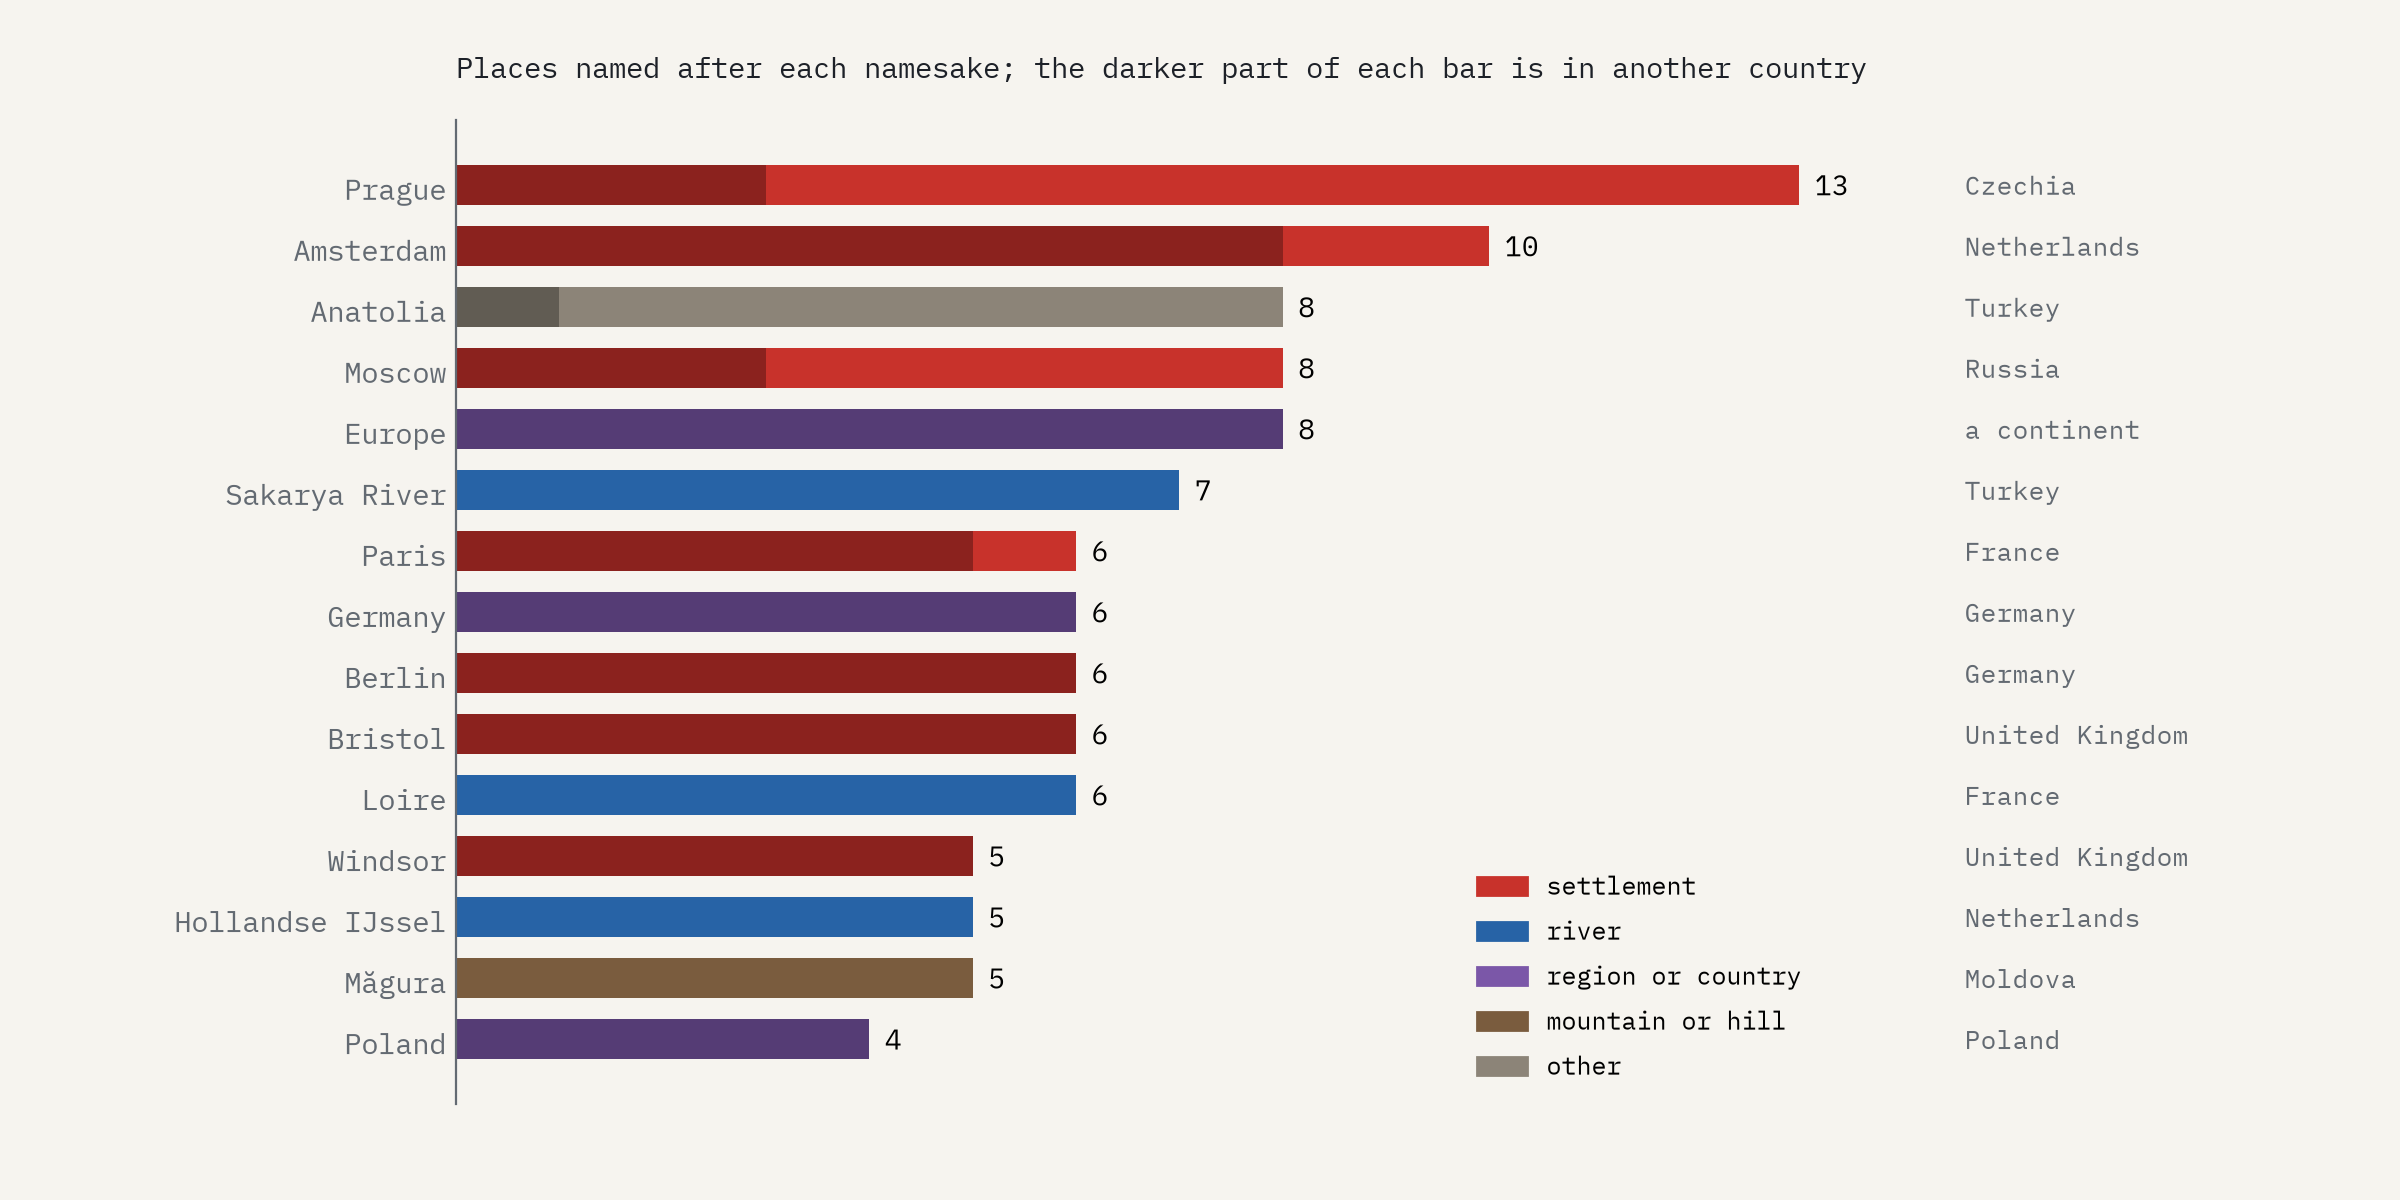
\includegraphics[width=.95\textwidth]{f_top.png}
\caption{The fifteen namesakes with the most places named after them; the darker part of each bar is in another country.}\label{fig:top}\end{figure}

\subsection{Who named whom}
881 links (22.1\%) cross a national border (Figure~\ref{fig:flows}, Table~\ref{tab:flows}). The United Kingdom gave 259 of them (29.4\%), followed by Germany (51), the Netherlands (42) and France (41). Of Britain's, 102 went to the United States, 102 to Australia, 31 to Canada and 13 to New Zealand, 95.8\% in all; Ireland added 21 to the same four countries. The United States received the most names from abroad (343), then Australia (138) and Canada (60). Grouping countries into ten regions, 58.1\% of border-crossing links run from one of the six European regions to North America, Latin America, or Asia and Oceania. Smaller flows trace particular histories: Dutch names in the former New Netherland (21 links from the Netherlands to the United States), and 12 Greek places named after places in Turkey, such as Nea Smyrni, settled by refugees in the 1920s. Flows in the opposite direction, from the Americas to the rest of the world, number 17.

The great Spanish and Portuguese naming of the Americas is almost absent. Spain and Portugal gave 34 names abroad in the file, only 6 of them to Latin America and 9 to the Philippines, and places in Latin America make up 2.2\% of all links. This is a gap in Wikidata's records, not in history.

\begin{table}[tbp]\centering\small\caption{The twenty largest country-to-country flows of names (links crossing a border).}\label{tab:flows}\begin{tabular}{llr}\toprule From (namesake) & To (place) & Links\\\midrule
United Kingdom & Australia & 102\\
United Kingdom & United States & 102\\
United Kingdom & Canada & 31\\
Germany & United States & 27\\
Netherlands & United States & 21\\
Italy & United States & 18\\
France & United States & 14\\
Spain & United States & 13\\
United Kingdom & New Zealand & 13\\
Canada & United States & 13\\
Turkey & Greece & 12\\
Norway & United States & 10\\
Belgium & Germany & 10\\
Ireland & United States & 10\\
Spain & Philippines & 9\\
Sweden & United States & 9\\
France & Canada & 9\\
Switzerland & United States & 9\\
Netherlands & Germany & 8\\
Ireland & Australia & 8\\
\bottomrule\end{tabular}\end{table}

\begin{figure}[tbp]\centering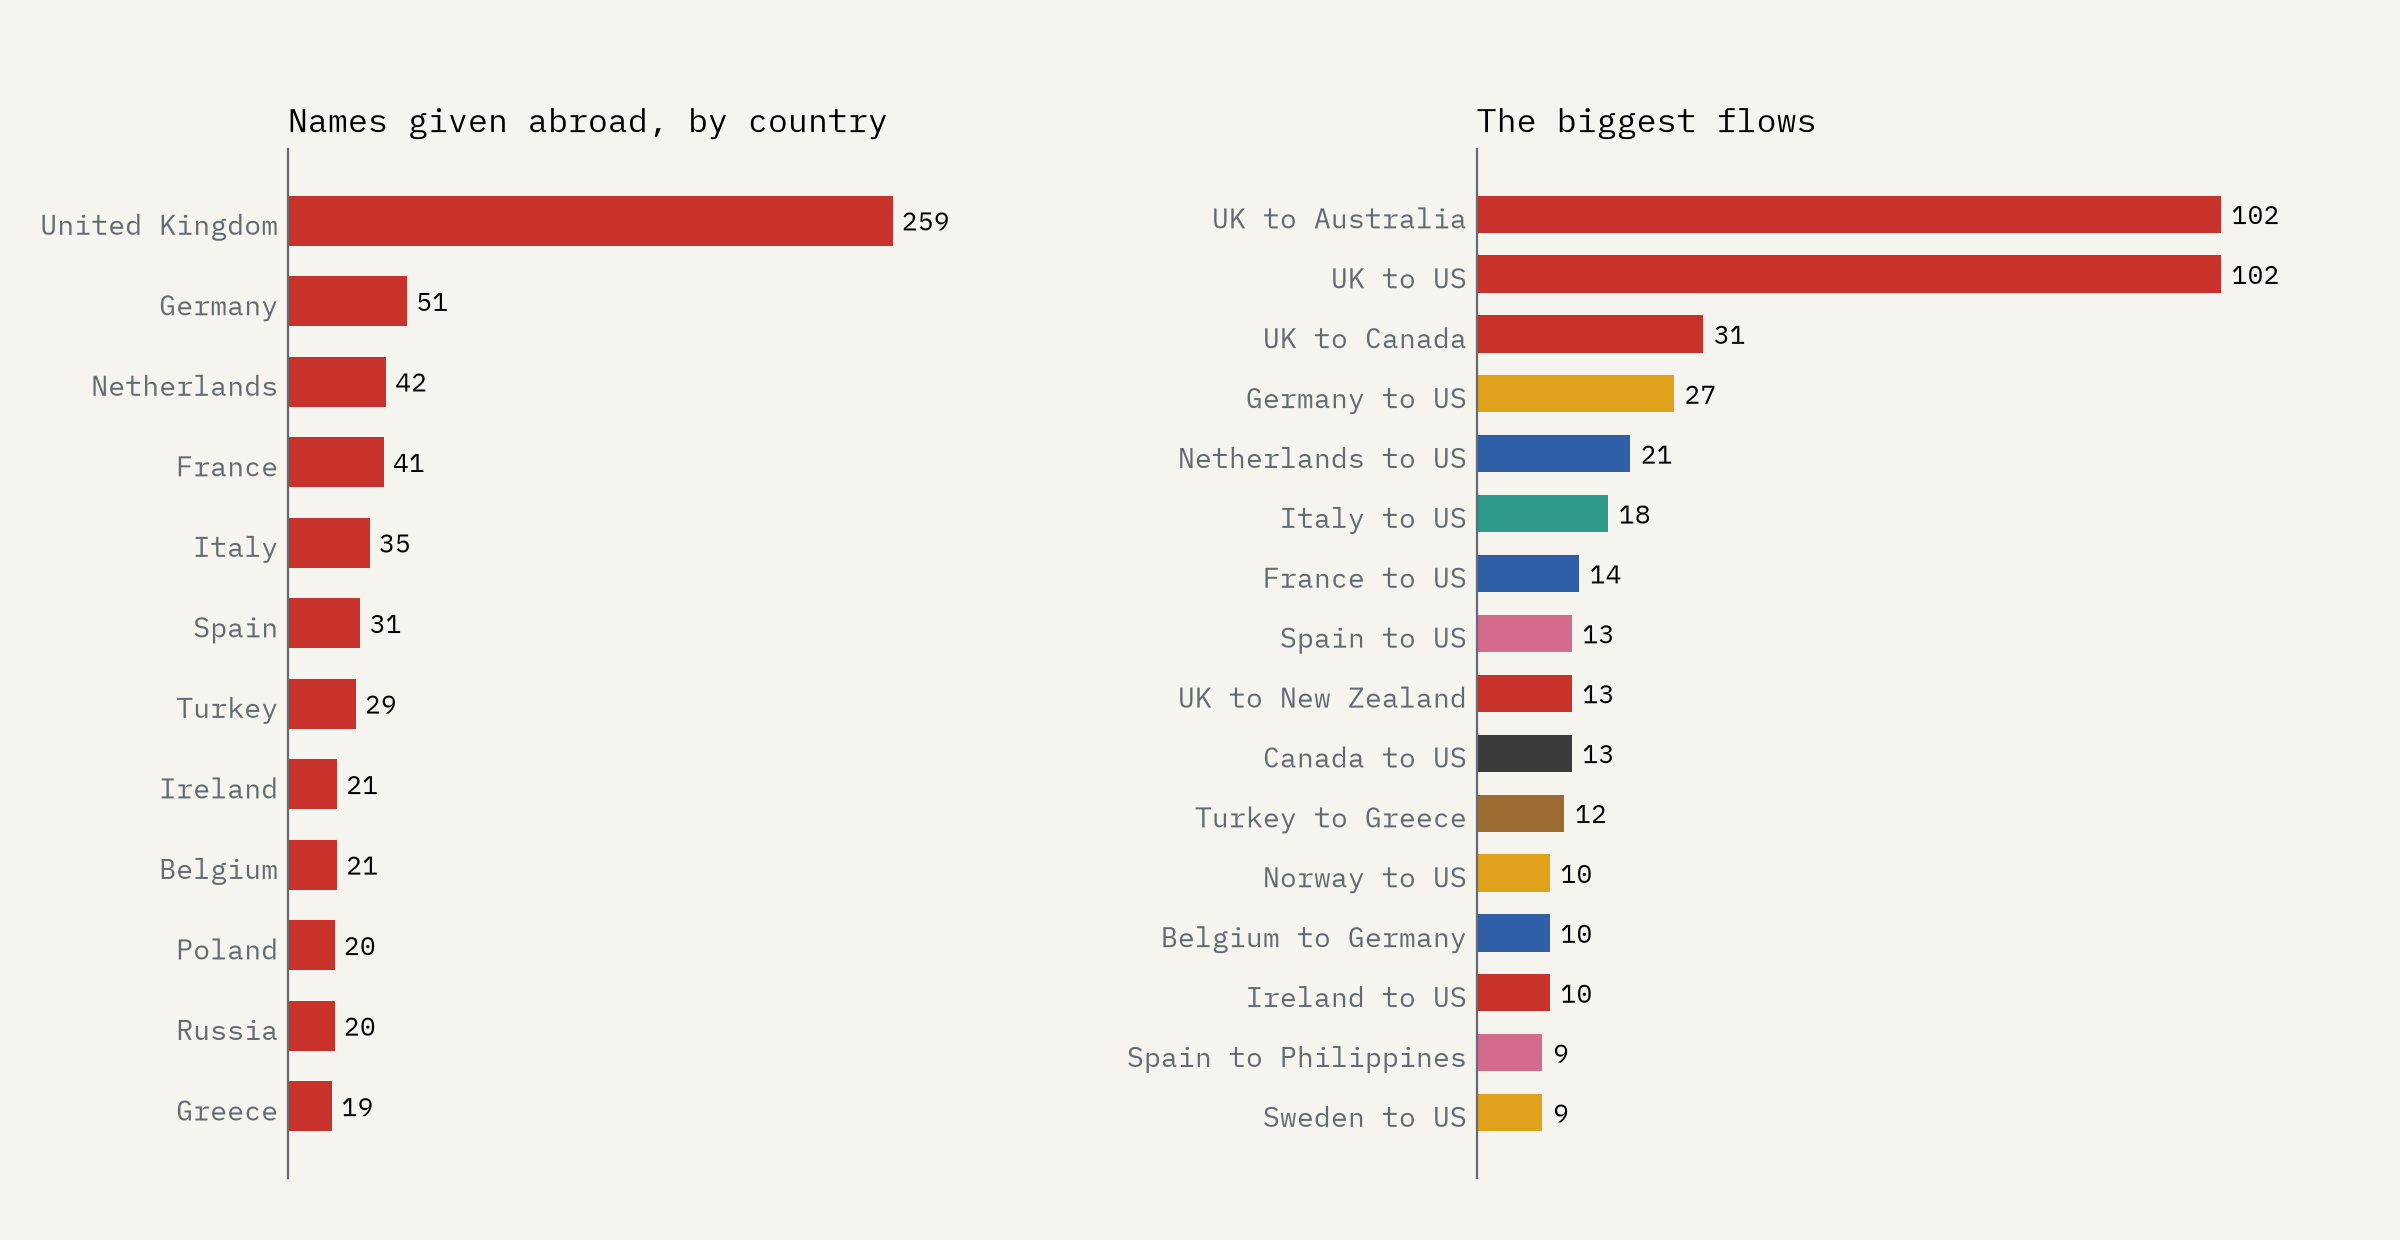
\includegraphics[width=\textwidth]{f_flows.png}
\caption{Left: names given across a border, by the namesake's country. Right: the largest country-to-country flows, coloured by the giving region.}\label{fig:flows}\end{figure}

\subsection{New X}
75 places have a name made of a word for new (New, Nieuw, Neu, Nova, Novo, Nueva and others) and the name of their namesake. Their median distance from the original is 15.1 km, and 54.7\% are within 30 km: Neu-Ulm across the Danube from Ulm, New Delhi beside Delhi, Dutch villages beside their older namesakes (14), German ones (12), and the new desert cities of Egypt (12). 18 crossed an ocean, among them New Amsterdam, New Madrid, Novo Hamburgo and Nueva Palmira.

\subsection{The Old World in the United States}
The United States has 998 links (25.1\% of the file), 343 to places abroad and 316 to places outside the Americas, in 47 states (Figure~\ref{fig:us}). Britain supplied 102 of the names from abroad, Germany 27 and the Netherlands 21. Classical names (Athens, Rome, Sparta, Ithaca, Syracuse and others) account for 14 links and names from the Holy Land and its neighbours for 14. Minnesota leads with 45, but 113 of Minnesota's 151 links are townships, which reflects bulk entry of township name origins into Wikidata rather than anything unusual about Minnesota.

\begin{figure}[tbp]\centering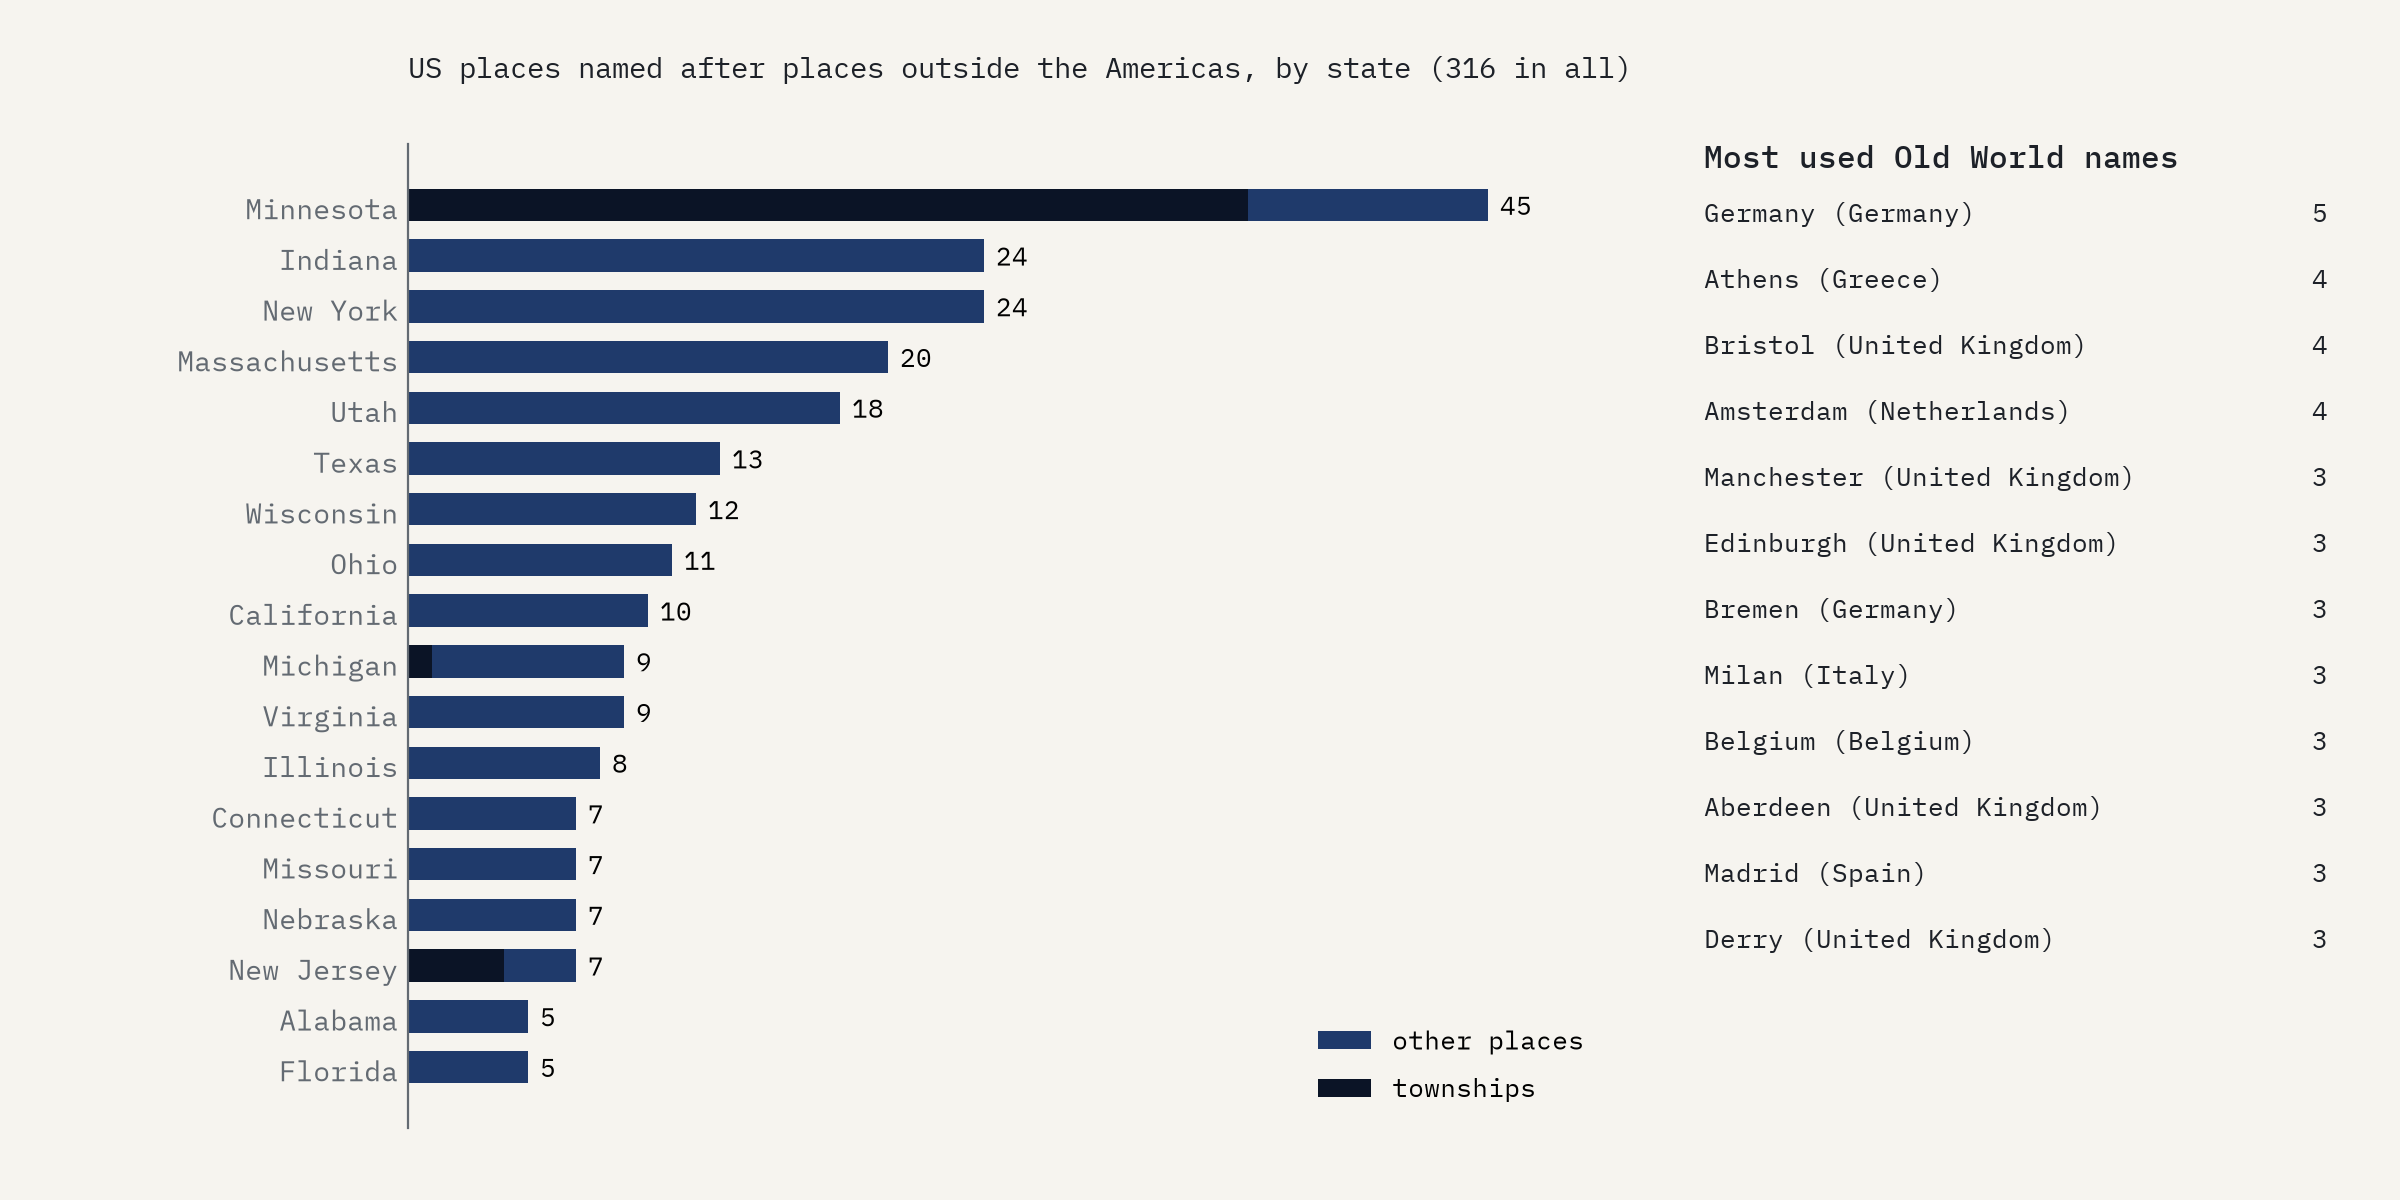
\includegraphics[width=\textwidth]{f_us.png}
\caption{US places named after places outside the Americas, by state, and the Old World names used most often.}\label{fig:us}\end{figure}

\subsection{Coverage}
The file is not a census of transferred names (Figure~\ref{fig:coverage}). Four countries, the United States (998), Germany (433), Australia (405) and the Netherlands (323), hold 54.2\% of links. The United Kingdom has 73, China 32, India 13, Brazil 40 and Mexico 1. Per person, the Netherlands has 18.6 links per million and India 1.0 per hundred million. 71 of the 160 countries with at least a million people have no links. Founding dates are given for 305 of the 881 places named after somewhere in another country; their median is 1856 (Figure~\ref{fig:founded}).

\begin{figure}[tbp]\centering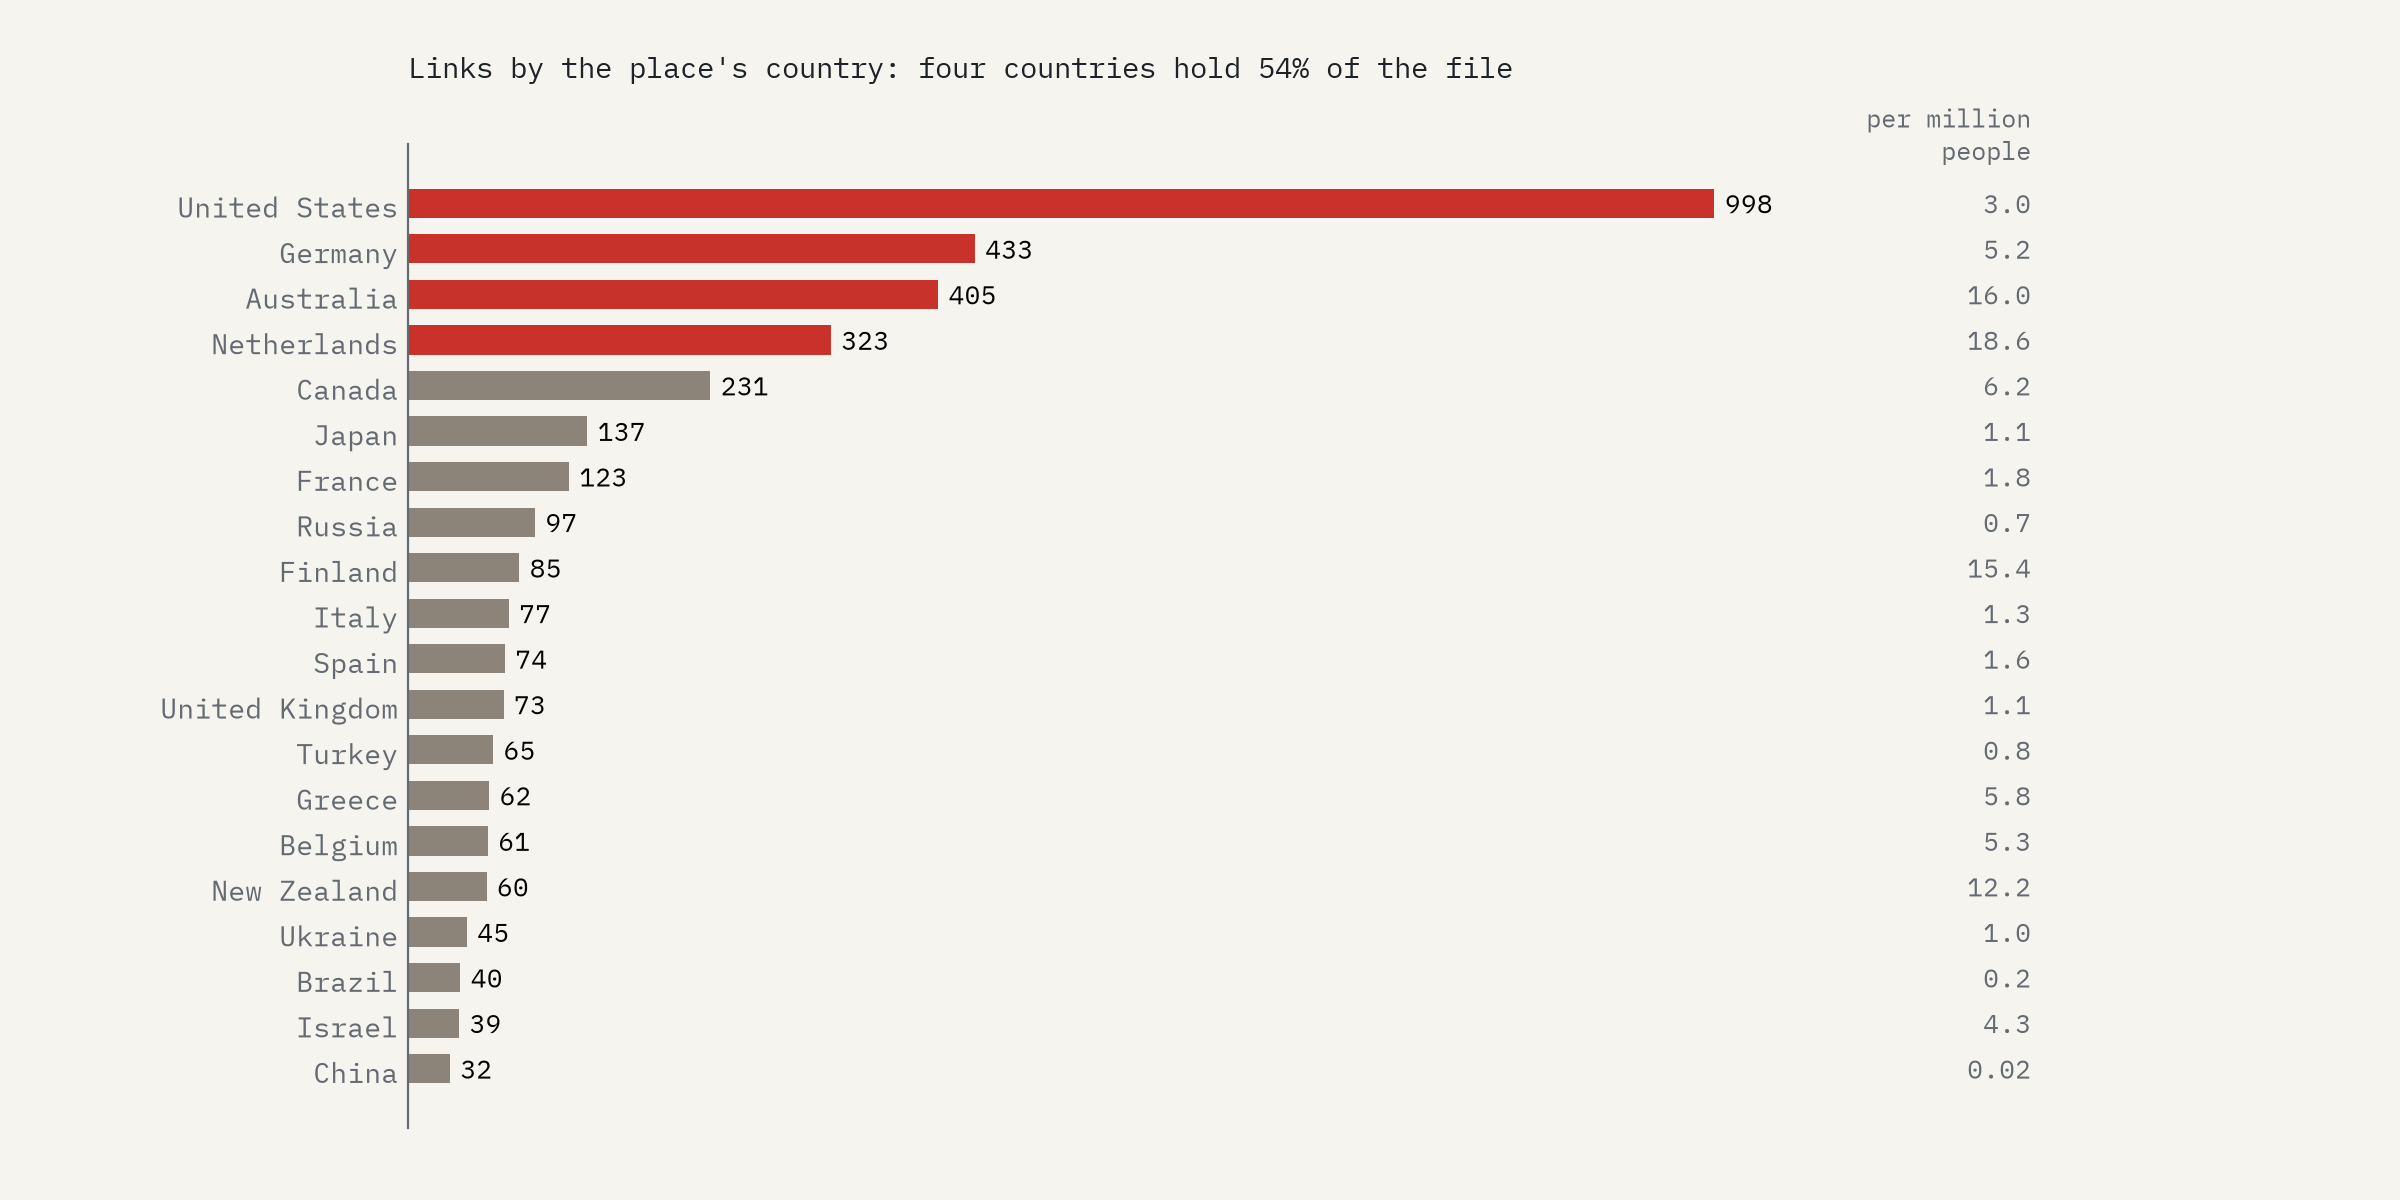
\includegraphics[width=.95\textwidth]{f_coverage.png}
\caption{Links by the place's country, with links per million people.}\label{fig:coverage}\end{figure}

\begin{figure}[tbp]\centering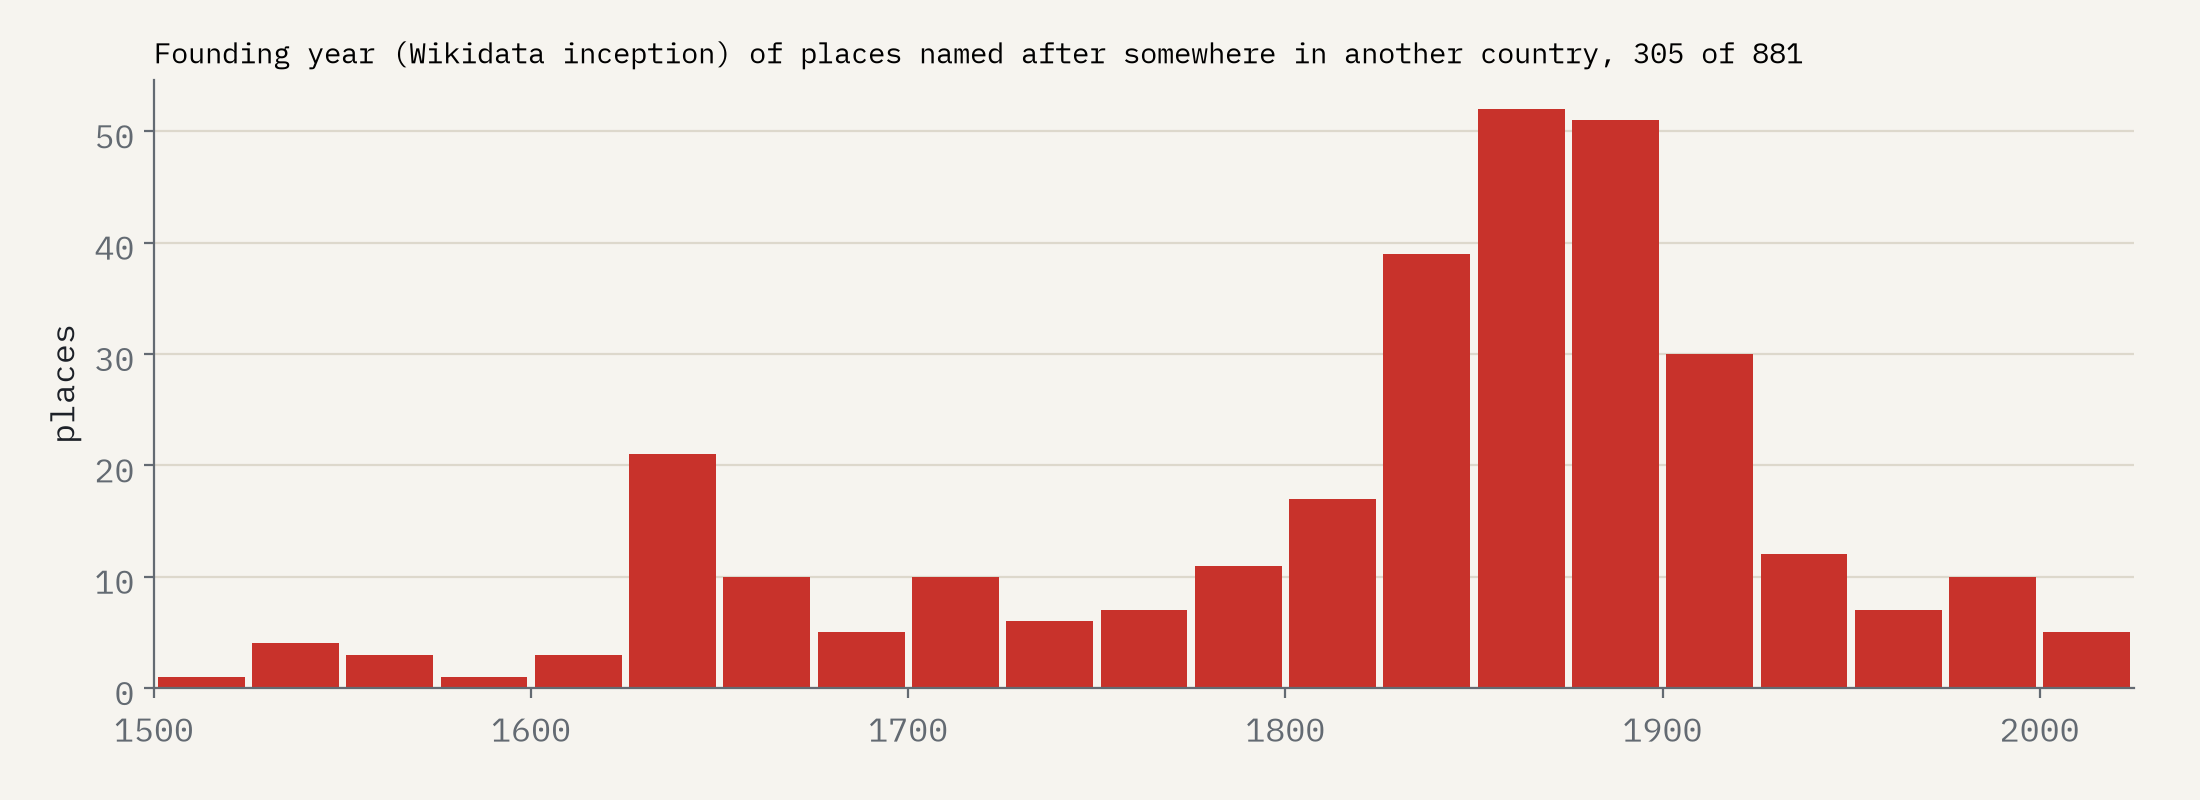
\includegraphics[width=.95\textwidth]{f_founded.png}
\caption{Founding year (Wikidata inception, in 25-year bins) of places named after somewhere in another country.}\label{fig:founded}\end{figure}

\section{Limitations}
First, Wikidata's ``named after'' statements are crowd-sourced and mostly unreferenced, and their coverage depends on editors and bulk imports rather than on the history of naming; the coverage section shows how uneven this is. Second, the query requires the namesake to be a geographic location with coordinates, so places named after people, saints, events or ships, and those whose namesake is a place without coordinates, are outside the study; New York City, for example, is not in the file. Third, the exclusion of non-settlements is by label and will have missed some items and removed a few that might be kept. Fourth, the categories rest on my reading of unlabelled class identifiers. Fifth, distances to rivers, regions and mountain ranges use a single point. Sixth, countries are present-day, so a link within the Soviet Union or the British Empire at the time of naming may appear as crossing a border today.

\section{Conclusion}
Most places that Wikidata records as named after another place took the name of something close by: a river, a hill, a lake, the town next door. The minority that carried a name across a border form a second, distinct population of long-distance transfers, dominated by British names in the United States, Australia, Canada and New Zealand, with smaller Dutch, German, Scandinavian and Greek streams. The file is best read as an early, partial atlas of transferred names, sharp where Wikidata is detailed and blank where it is not; as name origins are added for Latin America, Africa and Asia, the same method will show whether the British dominance holds.

\section*{Data and code availability}
The interactive map is at \url{https://maps.tristanhotham.com/named-after/}. Data and code are at \url{https://github.com/Tristan-Hotham/named-after} and archived with this paper at https://doi.org/10.5281/zenodo.23878606. Derived data and text are released under CC BY 4.0 and code under the MIT licence. Wikidata content is CC0.

\section*{AI statement}
I wrote the text, with drafting and editing assistance from Claude (Anthropic), which also helped prepare the analysis code. I reviewed and checked all text and results.

\begin{thebibliography}{9}
\bibitem[Wikidata(2026)]{wikidata} Wikidata contributors (2026) Wikidata. \url{https://www.wikidata.org/}. CC0. Queried in 2026.
\bibitem[Bast and Buchhold(2017)]{qlever} Bast, H. and Buchhold, B. (2017) QLever: a query engine for efficient SPARQL+Text search. In \textit{Proceedings of the 2017 ACM Conference on Information and Knowledge Management}, 647 to 656. \url{https://qlever.cs.uni-freiburg.de/}
\bibitem[Natural Earth(2026)]{naturalearth} Natural Earth (2026) Admin 0 countries, land, admin 1 states and provinces, and populated places. Public domain. \url{https://www.naturalearthdata.com/}
\end{thebibliography}
\end{document}
